\documentclass[11pt]{article}
\pdfinfoomitdate=1\pdftrailerid{}
\usepackage[letterpaper,margin=.7in,headheight=15pt,headsep=18pt,footskip=24pt]{geometry}
\usepackage[T1]{fontenc}
\usepackage{lmodern,amsmath,amssymb,array,booktabs,fancyhdr,tikz}
\usetikzlibrary{arrows.meta}
\renewcommand{\familydefault}{\sfdefault}
\setlength{\parindent}{0pt}\setlength{\parskip}{7pt}
\pagestyle{fancy}\fancyhf{}
\fancyhead[L]{\small Week 57 / Area from dots / K--1 adult guide}
\fancyfoot[L]{\scriptsize Bellingham Math Circle / Week 57 / N57-K-FAC-v1}
\fancyfoot[R]{\thepage}
\newcommand{\head}[1]{\par\textbf{\large #1}\par}
\newcommand{\sub}[1]{\par\textbf{#1}\par}
\newcommand{\hint}[1]{\textit{Only if needed:} #1}
\newcommand{\dotgrid}[2]{\foreach \x in {0,...,#1}{\foreach \y in {0,...,#2}{\fill (\x,\y) circle (1.25pt);}}}
\newcommand{\onestar}{\fill (0,0) circle (1.5pt);}
% #1-#4 indicate square (1) or inward-facing half (0), NE,NW,SW,SE.
\newcommand{\closer}[4]{%
  \foreach \r/\full in {0/#1,90/#2,180/#3,270/#4}{%
    \begin{scope}[rotate=\r]
      \ifnum\full=1\filldraw[fill=gray!18] (0,0) rectangle (1,1);
      \else\filldraw[fill=gray!18] (0,0)--(1,0)--(0,1)--cycle;\fi
    \end{scope}}
  \foreach \x in {-1,0,1}{\foreach \y in {-1,0,1}{\fill (\x,\y) circle (1.1pt);}}
  \draw (-.13,-.13) rectangle (.13,.13);}
\begin{document}
\head{Mathematical overview: paper, outline dots and inside dots}
\textbf{For one gap-free shape, outline dots plus twice the inside dots equal the number of halves plus two.} Count a square as two halves. Pieces lie flat without overlap, every corner is on the square lattice, and they join along whole sides into one shape. Exclude holes, corner-only connections and gaps pinched shut at a dot. Count \emph{all} outline dots, including those between corners, once each; this is not a count of corners or a length.

For adults, this is Pick's theorem in half-square units: $B+2I=H+2$, where $H=2A$. Thus with no inside dot there are two more outline dots than halves; for fixed paper, each extra inside dot means two fewer outline dots. The week's main guide, p.~1, gives the older bands' destination and assumptions; pp.~6--8 explain the general theorem. K--1 investigates these consequences with uncut pieces, not the general polygon proof or holes.

\textbf{Three pieces cannot close in a dot; four can.} Every lattice dot in a piece is a corner. A square or a half contributes at most a quarter-turn around it. Three quarter-turns leave a gap. Four right-angle corners can go all the way around. A child can place the corners, point to the missing quarter, and say why changing their positions will not make a bigger corner. This is an explanation, not just a failed search. For two neighboring dots, all six cells touching them need paper; one uncut piece cannot occupy two cells, so at least six pieces are needed.

\textbf{What children discover.} Rearranging equal amounts of paper can preserve a dot count, then closing in a dot changes it. A built shape and its marked drawing are an experiment; ``it always has five'' after several trials is a conjecture. A complete small catalog or an argument about the available corners explains a stated claim. The full dot rule is adult knowledge, not a formula children must learn. For a small growing shape with no dot enclosed, a new half sharing one side adds one outline dot; a closing corner changes the count. Let children notice the contrast before offering the rule.

\head{Preparation and access}
\textbf{Status.} Unpiloted and physically unrehearsed. Exact print scale, hand-cut piece fit, covered-dot visibility, tracing, handling by K--1 children, staffing and timing still need a real-material trial.

\textbf{Per pair.} Use the existing kit: 10 intact squares, each 20~mm on a side; 20 diagonal halves with 20~mm legs; 2 pencils, 1 eraser and 2 colored pencils (or circle/box marks). Keep the kit's scissors with the adult; no smaller pieces are allowed. A straightedge is available for adult tracing but is not a child prerequisite. Keep K--1 pieces apart from the older tables' cut duplicates. If kits are not already made, print \texttt{week-57-materials.pdf}, pp.~1--2, once on card stock: 60 squares and 120 halves give five kits, plus 10 squares and 20 halves spare. No new manipulative or unprinted board is needed.

\textbf{Print and prepare.} Print \texttt{k-1.pdf}, pp.~1--7, single-sided US Letter at Actual Size: 7 sheets per pair, 14 for two pairs; pp.~1--3 alone need 6 sheets for two pairs. Retain the week's older-band plan and one spare \texttt{week-57-students.pdf} p.~4 grid for the shared/table demonstration; the new packet replaces the younger pairs' independent work on those grids. Print one copy of this section for their adult. Beyond the week's kit preparation, allow an estimated 10--15 minutes to print, measure 20~mm intervals in both directions, compare a piece with the dots, and rehearse tracing. The materials' 100~mm bars also need measuring. Estimates are not rehearsal evidence.
\newpage
\head{Launch, pacing and the concrete core}
\textbf{Prerequisites and adult role.} No independent reading, fractions, letters or coordinates are needed. Children count pieces and dots to about 10 (up to 12 halves if recording the six-square solution), distinguish on/inside, and rotate pieces. Keep one adult anchored to the two K--1 pairs: read each question aloud and record the child's counts when asked. Children choose, place, classify and check. One partner can hold pieces while the other traces, then swap; the adult helps only where slipping prevents a recoverable outline. If every attempt needs adult tracing, preserve one shape per pair before resetting rather than make the adult run both investigations.

\textbf{After the whole-group launch.} Join the week's handling time and $2\times2$ square demonstration (main guide p.~3). At the table, use a spare 20~mm grid, not the miniature pictures at the top of K--1 p.~1. Place \emph{three squares in a straight row}, a non-task instance. Ask a child to touch a middle-of-side dot. Trace, lift, circle the outline dots, and show the two record icons: paper measured in halves; dots on the outline. This repeats the printed input--trace--mark convention without solving a numbered task.
\begin{center}
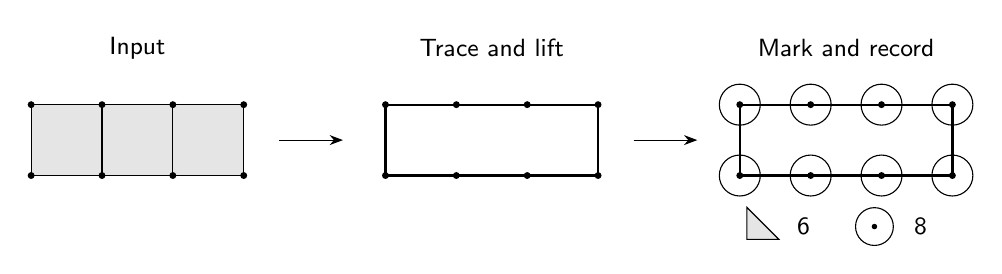
\begin{tikzpicture}[x=9mm,y=9mm,font=\small]
  \foreach \shift/\label in {0/Input,5/Trace and lift,10/Mark and record}{
    \node at (\shift+1.5,1.8) {\label};
    \begin{scope}[shift={(\shift,0)}]
      \ifnum\shift=0
        \foreach \x in {0,1,2}{\filldraw[fill=gray!20] (\x,0) rectangle ++(1,1);}
      \else\draw[thick] (0,0) rectangle (3,1);\fi
      \dotgrid{3}{1}
      \ifnum\shift=10
        \foreach \x in {0,1,2,3}{\foreach \y in {0,1}{\draw (\x,\y) circle (2.6mm);}}
        \filldraw[fill=gray!20] (.1,-.9)--(.55,-.9)--(.1,-.45)--cycle;
        \node at (.9,-.72) {6};
        \fill (1.9,-.72) circle (1pt);\draw (1.9,-.72) circle (2.4mm);
        \node at (2.55,-.72) {8};
      \fi
    \end{scope}}
  \draw[-{Stealth}] (3.5,.5)--(4.4,.5);
  \draw[-{Stealth}] (8.5,.5)--(9.4,.5);
\end{tikzpicture}
\end{center}
\textbf{Keep the rules visible.} The page~1 yes/no pictures distinguish a whole-side join from a corner-only contact. The entire shape must connect through sides; opposite pieces may still meet at a corner. Stars on pp.~4--6 are targets, not assertions that a dot is already inside. Trace and lift before deciding: cracks or the star's ink showing through are not reliable geometric tests. Include gaps that open only at a single dot in ``no gap inside.''

\textbf{A first hour.} Use the week's 0--10 minute movement/handling/shared launch. Allow 10--13 for the table demonstration, 13--25 for P1 and 25--35 for P2. After the week's 35--38 reset, choose P3 or continue P2 until the children own the choices. At 50--57 share one kept shape and one conjecture; tidy and note the next starting point by 60. Save P4--5 for a return, or offer them to a ready pair; P6--7 need the one-dot work first. Finishing every page is not the goal.

\sub{Problem 1, student page 1: six covers}
In reading order, the records (halves, outline dots) are
\[
(1,3),\ (2,4),\ (2,4),\ (2,4),\ (4,6),\ (4,6).
\]
No dot is inside any of these shapes. Cover, trace if needed, lift and count each dot once. In the wide triangle and bottom trapezoid, a dot halfway along a straight side counts too. The paper amount stays the same in each contrasting pair even when the outline looks different. \hint{``Which dots sit on the line even though the line does not turn there?'' ``Can two halves cover the same space as that square?''}

\sub{Problem 2, student page 2: three halves}
\textbf{No: every allowed shape has five outline dots and none inside.} Three pieces cannot surround a dot; the overview's dot rule then gives five. In concrete joins, a first half has three dots and each of the next two brings one new outline dot. The checker exhausts the possibilities independently. There is no requirement to find six \emph{different} shapes or fill all six boards; repeats are useful tests. \hint{``Did any dot end up inside?'' ``Is that a whole-side join?''} Keep ``always five'' as a conjecture if the child has only tried examples.
\newpage
\head{A dot moves inside}
\sub{Problem 3, student page 3: four halves}
\textbf{The fewest is four outline dots}, attained by the tilted square below, with one inside dot. Any other shape has six outline dots and none inside. An independent exhaustive check gives 14 shapes up to turns and flips: 13 of the latter kind and this one. This is an adult completeness check, not a demand to draw all 14 on six boards. All fit the printed $3\times4$-dot boards after turning.
The first picture in P5's strip below shows it: four halves meet with their right angles at the middle dot. Circle the four outer dots and box the middle one.

Why no smaller outline count? Four halves have room for at most one inside dot: two inside dots require paper in at least six distinct unit cells (even when the dots are farther apart), hence at least six pieces. The dot rule gives four or six. \hint{``Can any dot become completely surrounded?'' ``What happened to the outline count when it did?''} If the pair finds the tilted square early, compare it with one of its six-dot drawings rather than request more routine examples.

\sub{Problem 4, student page 4: three pieces around the star}
\textbf{Impossible, whether the pieces are squares or halves.} At the star each piece can fill at most a right-angle corner. Three leave at least one quarter-turn empty; a half's sharp corner fills even less. Let children put their largest corners around the star and point to what is missing. This rules out all positions, unlike repeated unsuccessful attempts. The $5\times5$-dot board does not require filling its whole frame. \hint{``Which corner covers the most space next to the star?'' ``Do three such corners go all the way around?''} A natural continuation is to ask what one more piece could change, then offer P5.

\sub{Problem 5, student page 5: all four-piece closers}
\textbf{Six shapes}, with a turned copy counted as the same, exactly as printed. Each of the four pieces must contribute a right angle at the star: a square or a half with its \emph{square corner} there. This leaves four surrounding cells, each with those two choices. The table is the complete list; all fit the $3\times3$-dot boards.
\begin{center}
\renewcommand{\arraystretch}{1.16}
\begin{tabular}{lccc}
Squares among the four pieces & Half pieces & Paper in halves & Outline dots\\\midrule
None & 4 & 4 & 4\\
One & 3 & 5 & 5\\
Two, next to each other & 2 & 6 & 6\\
Two, opposite each other & 2 & 6 & 6\\
Three & 1 & 7 & 7\\
Four & 0 & 8 & 8
\end{tabular}

\vspace{3mm}
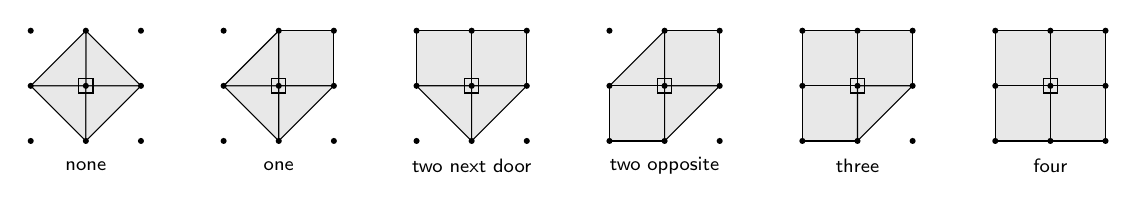
\begin{tikzpicture}[x=7mm,y=7mm,font=\scriptsize]
\begin{scope}[shift={(0,0)}]\closer{0}{0}{0}{0}\node at (0,-1.45) {none};\end{scope}
\begin{scope}[shift={(3.5,0)}]\closer{1}{0}{0}{0}\node at (0,-1.45) {one};\end{scope}
\begin{scope}[shift={(7,0)}]\closer{1}{1}{0}{0}\node at (0,-1.45) {two next door};\end{scope}
\begin{scope}[shift={(10.5,0)}]\closer{1}{0}{1}{0}\node at (0,-1.45) {two opposite};\end{scope}
\begin{scope}[shift={(14,0)}]\closer{1}{1}{1}{0}\node at (0,-1.45) {three};\end{scope}
\begin{scope}[shift={(17.5,0)}]\closer{1}{1}{1}{1}\node at (0,-1.45) {four};\end{scope}
\end{tikzpicture}
\end{center}
With zero, one, three or four squares, rotation leaves just one case. With two, they are neighbors or opposites. These cannot turn into each other; there are no other cases. Flipping adds none either. Every record has one inside dot; the paper-in-halves and outline counts agree. Count a square as \emph{two}, not one, beside the half icon. Nine boards allow retries, not nine required answers. \hint{``Can you turn one saved picture onto another?'' ``Where could the two squares sit?''} Let pairs pool their kept pictures before the adult organizes them into this catalog.
\newpage
\head{Two inside dots and less outline}
\sub{Problem 6, student page 6: both stars, fewest pieces}
\textbf{Six pieces are necessary and sufficient.} The stars are horizontally adjacent on the $6\times5$-dot board. A $3\times2$ rectangle made from six whole squares encloses both; its paper is worth 12 halves and it has ten outline dots. The roofed hexagon below uses two squares and four halves: still six \emph{pieces}, but only eight halves of paper and six outline dots. Both are valid answers to the fewest-pieces question.

\textbf{Why five cannot work.} Each star needs paper in all four cells touching it. The two stars share two cells, so six distinct cells must be occupied. Every allowed uncut piece stays within a single unit cell; one piece cannot cover two of those cells. Six are therefore necessary. With exactly six pieces the two shared cells must hold squares: a half cannot supply full right-angle corners at both stars. The four outside cells may each hold a square or an inward-pointing half. This describes every six-piece solution without asking children to enumerate them.

\hint{``Which spaces right next to each star must have paper?'' ``Can one of our pieces reach into two different little squares?''} Use the six-square rectangle as an adult rescue only after a real search. Children who find a six-piece construction have established that six works; ask for the lower-bound explanation only when their cell distinction is secure. Save a traced outline for the next question.

\sub{Problem 7, student page 7: eight halves, fewer outline dots}
The printed $2\times2$ square uses eight halves and has eight outline dots and one inside dot. \textbf{Exactly two shapes, up to turns and flips, improve on eight: both have six outline dots and two inside dots.} They fit either $4\times5$-dot workboard. The task asks for one; finding the other is a natural continuation, not an extra first-visit demand.
\begin{center}
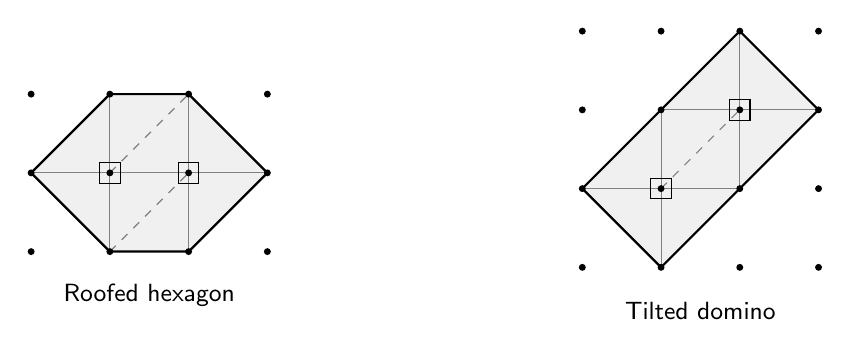
\begin{tikzpicture}[x=10mm,y=10mm,font=\small]
\begin{scope}
  \filldraw[fill=gray!12,thick] (0,1)--(1,0)--(2,0)--(3,1)--(2,2)--(1,2)--cycle;
  \draw[gray] (1,0)--(1,2) (2,0)--(2,2) (0,1)--(3,1);
  \draw[dashed,gray] (1,0)--(2,1) (1,1)--(2,2);
  \dotgrid{3}{2}
  \foreach \x in {1,2}{\draw (\x-.13,.87) rectangle (\x+.13,1.13);}
  \node at (1.5,-.55) {Roofed hexagon};
\end{scope}
\begin{scope}[shift={(7,-.2)}]
  \filldraw[fill=gray!12,thick] (1,0)--(3,2)--(2,3)--(0,1)--cycle;
  \draw[gray] (0,1)--(2,1) (1,0)--(1,2) (1,2)--(3,2) (2,1)--(2,3);
  \draw[dashed,gray] (1,1)--(2,2);
  \dotgrid{3}{3}
  \foreach \p in {1,2}{\draw (\p-.13,\p-.13) rectangle (\p+.13,\p+.13);}
  \node at (1.5,-.55) {Tilted domino};
\end{scope}
\end{tikzpicture}
\end{center}
These compact adult pictures show the outer outlines and piece divisions. Dashed lines split square regions into halves; \emph{P7 uses eight half pieces, not intact squares}. In the tilted domino, each long slanted side has a middle dot to count. These are adult answer pictures, not piece-fitting templates.

The independent search checks every side-connected region of eight halves, rejecting gaps and pinched boundaries. It finds only these two with fewer than eight outline dots; their areas are also checked by the polygon coordinates, not inferred from the dot rule. \hint{``Could more than one dot end up inside?'' ``Can you cover your saved six-piece shape with halves instead?''} If a child joins two tilted squares only at a tip, there are two side-connected groups, not one legal shape. If a gap closes only at a corner, it is still a gap: trace and lift rather than trusting which ink the pieces hide.

\textbf{Keep for the next visit.} Save a marked drawing and the child's explanation or exact conjecture. Record where adult reading/recording was enough and where adult choices were needed. Geometry and exhaustive checks do not establish classroom readiness.

\textbf{Where it goes.} On approval, this section replaces ``K--1 route, outside the numbered packet'' on p.~3 of \texttt{week-57-facilitator.pdf} (W57-FAC-v4); its p.~1 K--1 pointer and p.~2 younger print quantities will also need updating at integration. The shared launch and older-band routes remain. Source context and teaching precedents stay in the main guide, p.~10; this section's counts are independently rechecked against N57-K-v1.
\end{document}
